\documentclass[a4paper,12pt,oneside ]{article}

\usepackage[utf8]{inputenc}
\usepackage[T1]{fontenc}      
\usepackage[francais]{babel}

\usepackage{graphicx}

\title{LFSAB1403 : DJ'Oz}
\author{Edward \bsc{Nicol} (27101300) \\ Virgile \bsc{Goyens}(83391300)}
\date{\today}

\begin{document}
\maketitle

\begin{figure}[h]
\begin{center}
	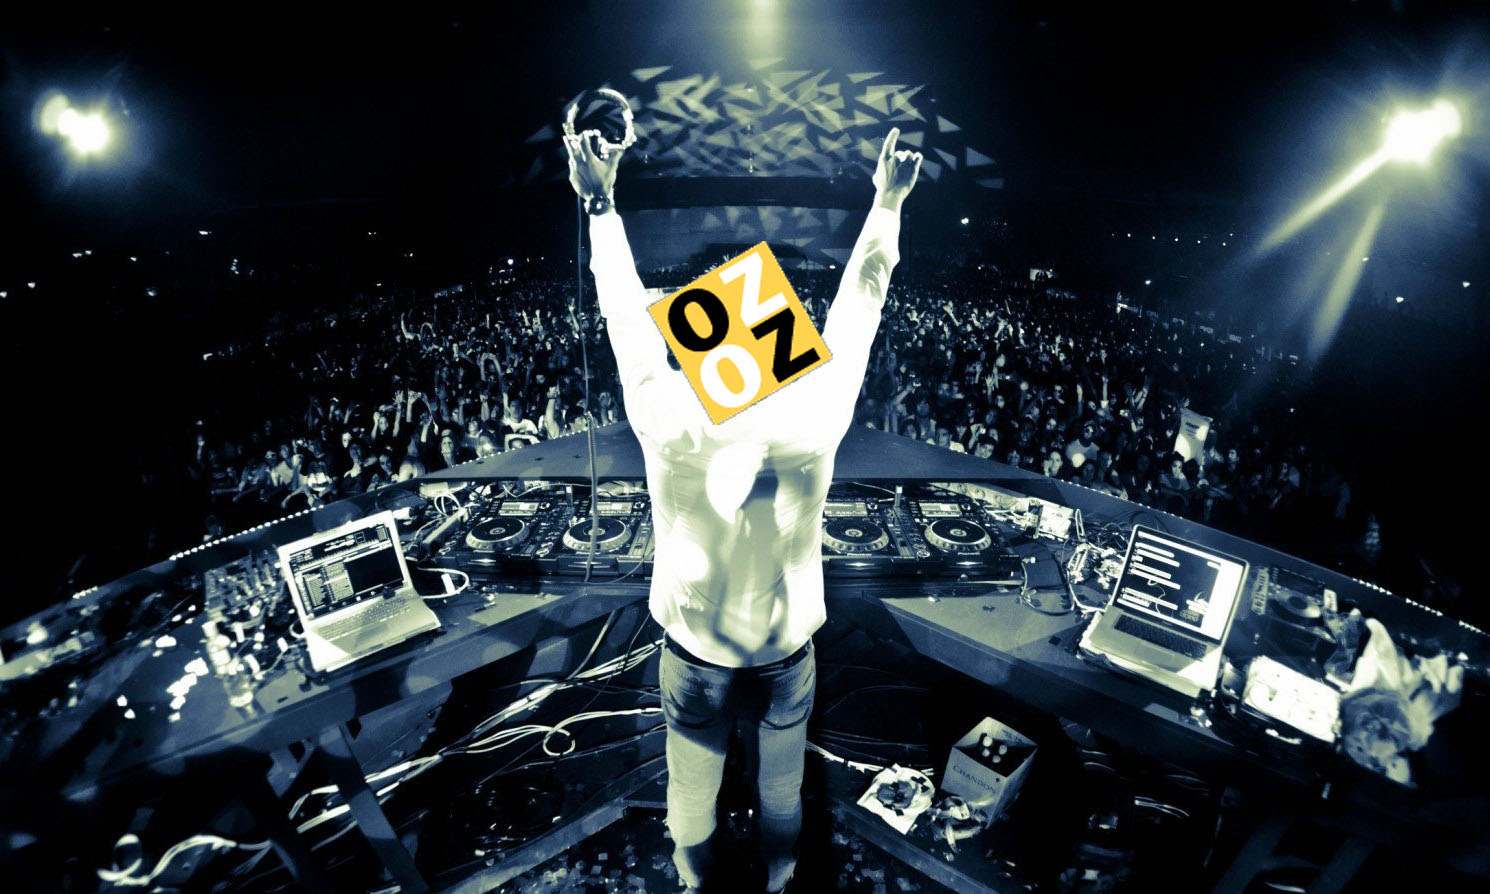
\includegraphics[scale=0.3]{DJOZ}
\end{center}
\end{figure}

\newpage
\section{Structure du programme}
	Le programme est divisé en deux grandes fonctions: la fonction \texttt{fun \{Interprete Partition\}} et la fonction \texttt{fun \{Mix Interprete Music\}}.
	
	Traitons dans un premier temps la fonction \texttt{fun \{Interprete Partition\}}. Cette fonction prend une partition comme argument et renvoie une voix, c'est à dire une liste d'échantillons. Cette fonction possède trois fonction locales: \texttt{fun\{ToNote Note\}}, \texttt{fun\{CountNotes Partition Acc\}}, \texttt{fun\{GetEchantillon Note Facteur Transposer\}} et fun \texttt{\{SuperInterprete Partition Bourdon Facteur Transposer\}}.
	
	Les 3 premières sont des fonctions utilisées dans le programme. \texttt{\{ToNote\}} permet d'uniformiser le format des notes. \texttt{\{CountNotes\}} permet de compter le nombre de notes d'une partition (utile dans le cas d'une transformation du type \texttt{duree()}). Finalement, \texttt{\{GetEchantillon\}} renvoie un échantillon d'une note quelconque, en prenant en compte plusieurs paramètres.
	
	La fonction \texttt{\{SuperInterprete\}} quant à elle représente le corps de la fonction. Grâce à ses paramètres supplémentaires, elle permet de tenir compte des modifications à apporter lors de la création d'un échantillon (du point de vue de la durée et/ou de la hauteur de la note. Elle utilise le principe du pattern matching pour interpréter la liste partition. Premièrement, un appel à la fonction \texttt{\{Flatten\}} est effectué pour ne plus avoir de liste imbriquées. Ensuite, pour chaque élément de la partition que la fonction rencontrera, elle vérifiera s'il s'agit d'une modification: le cas échéant, elle effectuera une modification dans les paramètres de la fonction \texttt{\{SuperInterprete\}}. Sinon, la fonction considérera que l'élément de partition est une note: elle fera donc appel à la fonction \texttt{GetEchantillon} et un appel récursif sera fait sur la queue de la liste. Le cas ou la partition ne comporte qu'un élément est aussi pris en compte.
	
	La fonction \texttt{fun\{Mix Interprete Musique\}} prend en argument la fonction \texttt{Interprete} que nous venons de d'écrire et une Musique qui peut prendre différentes formes. Nous départageons les différents cas grâce au pattern matching.
	
	La musique peut donc être une voix (qui est une liste d'échantillons), dans ce cas nous pouvons directement transformer notre échantillon en un vecteur audio qui a une taille de 44100 pour un échantillon de 1 seconde et dont les valeurs dépendent de la fréquence de l'échantillon. Elle peut aussi être une partition dans ce cas il suffit d'appliquer la fonction Interprete sur la partition pour la transformer en voix et ensuite la transformer en vecteur audio. 
	
	La fonction Mix gère également quelques filtres: \texttt{repetition},\texttt{clip},\texttt{couper},\texttt{echo}, \texttt{fondu} et \texttt{fondu\_enchaine}. Elles sont toutes basées sur le même principe qui consiste à modifier un certain vecteur audio en fonction des paramètres entrés et ensuite d'effectuer un appel récursif sur le reste de la musique.
	
	Nous avons eu pas mal de difficultés au début du projet lorsque nous avons du visualiser la tâche et donner une structure. Il n'a pas été facile de s'y retrouver entre tous les différents types utilisés, leur construction, ce pour quoi ils était utilisés... Aussi, la manière de traiter les cas de transformations pour \texttt{Interprete} et de filtres dans \texttt{Mix} n'a pas été instinctive.
	
\section{Constructions déclaratives}



\end{document}